%! Mode:: "TeX:UTF-8"
%! TEX program = xelatex
\PassOptionsToPackage{quiet}{xeCJK}
\documentclass[withoutpreface,bwprint]{cumcmthesis}
\usepackage{multirow}
\usepackage{CJKutf8}
\usepackage{ctex}
\usepackage{enumerate,mdwlist}
\usepackage{graphicx}
\usepackage{amsmath}
\usepackage{hyperref}
\usepackage{xcolor}
\usepackage{graphicx}
\usepackage{wrapfig}
\usepackage{lscape}
\usepackage{rotating}
\usepackage{epstopdf}
\hypersetup{
        colorlinks=false,
        linkbordercolor=red
    }
\usepackage{svg}

\usepackage{amsthm}
\usepackage{amsfonts}
\usepackage{enumitem}
\usepackage{mathpazo}
\usepackage{mathrsfs}
\usepackage{mathtools}
\usepackage{mathabx}
\usepackage{quiver}
\usepackage{hyperref}
\usepackage{IEEEtrantools}
\usepackage{physics}
\usepackage{etoolbox}
\BeforeBeginEnvironment{tabular}{\zihao{-5}}
\usepackage[numbers,sort&compress]{natbib}  % 文献管理宏包withoutpreface,
\usepackage[framemethod=TikZ]{mdframed}  % 框架宏包
\usepackage{url}  % 网页链接宏包
\usepackage{subcaption}  % 子图宏包
\newcolumntype{C}{>{\centering\arraybackslash}X}
\newcolumntype{R}{>{\raggedleft\arraybackslash}X}
\newcolumntype{L}{>{\raggedright\arraybackslash}X}

\newcommand{\fm}[5]{%function map
  \begin{tikzcd}[
    column sep=2em,
    row sep=1ex,
    ampersand replacement=\&
  ]
  #1\colon \&[-3em]
  #2\vphantom{#3} \arrow[r] \&
  #3\vphantom{#2} \\
  \&
  #4\vphantom{#5} \arrow[u,symbol=\in] \arrow[r,mapsto] \&
  #5\vphantom{#4} \arrow[u,symbol=\in]
  \end{tikzcd}%
}

\title{无人机协同避障航迹规划}  % 论文标题
\author{赖毅}
\author{车天石}

\schoolname{吉林大学}  % 学校
\membera{车天石}  % 队员a
\memberb{赖毅}  % 队员b
%%%%%%%%%%%%%%%%%%%%%%%%%%%%%%%%%%%%%%%%%%%%%%%%%%%%%%%%%%%%%




%% 正文
\begin{document}




\maketitle
\begin{abstract}
摘要

\textbf{对于问题一,}

\textbf{对于问题二,}

\textbf{对于问题三,}

\textbf{对于问题四,}

最后,



\keywords{关键词\quad  关键词\quad  关键词\quad  关键词 \quad 关键词}
\end{abstract}
%%%%%%%%%%%%%%%%%%%%%%%%%%%%%%%%%%%%%%%%%%%%%%%%%%%%%%%%%%%%% 
%%%%%%%%%%%%%%%%%%%%%%%%%%%%%%%%%%%%%%%%%%%%%%%%%%%%%%%%%%%%%  
\section{问题重述}
\subsection{背景}
我们将在重述问题中建立起最优控制的模型:

选取 30m为公度后, 把两台无人机看作是复平面上的质点$z_A,z_B$. 它们的初始位置在实轴上 $z_A(0)=(x_A,0), z_B(0)=(-350/3,0).$ 其中$x_A$恒为$[100/3,500/3]$中的一个值. 质点的运动速度大小均恒定, 分别为$v_A$和$1$, 其中 $v_A$恒为$[1/3,1]$中的一个值. 用哈密顿力学的眼光去看, 系统的相空间似乎为 $$\mathbb{C}\times \mathbb{C} \times v_A S^1 \times S^1 \subset \mathbb{R}^8$$

但是, 现实所要求的坐标空间要更为复杂. 首先, 障碍圆的存在要求 \[ |z_A|,|z_B| \geq (\frac{50}{3})^2, \] 其次, 两机不能碰面要求 \[ \frac{1}{2}\frac{|\Im(z_1\bar{z_2})|}{|z_1-z_2|} \leq \frac{50}{3}, \] 因为这等价于要求原点到直线的距离(也就是两个坐标向量张成的面积的一半除以两点的距离)不超过障碍圆的半径.

如果记 
% https://q.uiver.app/#q=WzAsNCxbMCwwLCJGOihcXG1hdGhiYntDfS01MC8zXFxtYXRoYmJ7RH0pXjIiXSxbMSwwLCJcXG1hdGhiYntSfV97XFxnZXEgMH0iXSxbMCwxLCIoeF8xLHlfMSx4XzIseV8yKSJdLFsxLDEsIlxcZnJhY3soeF8xeV8yLXhfMnlfMSleMn17KHhfMS14XzIpXjIrKHlfMS15XzIpXjJ9Il0sWzAsMV0sWzIsMywiIiwwLHsic3R5bGUiOnsidGFpbCI6eyJuYW1lIjoibWFwcyB0byJ9fX1dXQ==
\[\begin{tikzcd}
	{F:(\mathbb{C}-50/3\mathbb{D})^2} & {\mathbb{R}_{\geq 0}} \\
	{(x_1,y_1,x_2,y_2)} & {\frac{(x_1y_2-x_2y_1)^2}{(x_1-x_2)^2+(y_1-y_2)^2}}
	\arrow[from=1-1, to=1-2]
	\arrow[maps to, from=2-1, to=2-2]
\end{tikzcd}\]

那么系统的坐标空间为 \[ F^{-1}\mathbb{R}_{\geq 0}, \]
可见相空间的几何相当复杂, 似乎难以用变分法来求解. 

对于任一质点$i\in\{A,B\}$, 如果记其速度向量的方向为 $e^{i\theta_i}$, 则加速度向量为 \[ \vec{a}_i = v_i \dot{\theta}_i e^{i(\theta_i+\pi/2)}=\frac{v_i^2}{R_i} e^{i(\theta_i+\pi/2)} \]

由于\[ R_i\geq 1, \]
有\[ |\vec{a}_i|\leq v_i^2, \]
\[ -v_i \leq \theta_i \leq v_i. \]
特别的, 对于B机来说, 由于其速率恒定为$1$, 加速度大小与角速度大小等同, 上界均为$1$. 

对于操纵无人机的人, 或者说相空间的上帝来说, 可以控制的仅有以下变量: 初始速度向量的方向 
\[ \theta_A,\theta_B \in [-\pi,\pi] \]
和每一时刻的角速度(手柄没有前后, 仅有左右) 
\[ \dot\theta_A: [0,T]\to [-v_A,v_A] \]
\[ \dot\theta_B: [0,T]\to [-1,1]. \]

将上述控制变量编号为 $u_1,\dots,u_4$

%%%%%%%%%%%%%%%%%%%%%%%%%%%%%%%%%%%%%%%%%%%%%%%%%%%%%%%%%%%%% 

% \subsection{问题要求}

% \textbf{问题1}  

% \textbf{问题2}  

% \textbf{问题3} 

% \textbf{问题4}  

%%%%%%%%%%%%%%%%%%%%%%%%%%%%%%%%%%%%%%%%%%%%%%%%%%%%%%%%%%%%% 

\subsection{问题分类}
\subsubsection{$\text{min}_{u_i}\text{min}_{A,B}t$}

\begin{table}[H]
\centering
\begin{tabularx}{\textwidth}{CLC}
\toprule
问题    & x_A    & v_A \\
\midrule
一& $100/3$ & $1$ \\
三& $[50/3,+\infty]$ & $1$ \\
四& $100/3$ & $[1/3,1]$ \\
五& $[100/3,500/3]$ & $[1/3,1]$ \\
\bottomrule
\end{tabularx}
\label{tab:符号说明}
\end{table}
其中我们对问题三只讨论 $x_A$区间非平凡部分.(在障碍圆中显然无意义; 在负半轴上则与$B$碰面了. )
\subsubsection{$\text{min}_{u_i}\text{max}_{A,B}t$}
\begin{table}[H]
\centering
\begin{tabularx}{\textwidth}{CLC}
\toprule
问题    & x_A    & v_A \\
\midrule
二& $100/3$ & $1$ \\
三& $[50/3,+\infty]$ & $1$ \\
四& $100/3$ & $[1/3,1]$ \\
五& $[100/3,500/3]$ & $[1/3,1]$ \\
\bottomrule
\end{tabularx}
\label{tab:符号说明}
\end{table}

%%%%%%%%%%%%%%%%%%%%%%%%%%%%%%%%%%%%%%%%%%%%%%%%%%%%%%%%%%%%% 

% \section{模型假设}

% 为简化问题,本文做出以下假设:

% \begin{itemize}[itemindent=2em]
% \item 假设1
% \item 假设2
% \item 假设3
% \end{itemize}

%%%%%%%%%%%%%%%%%%%%%%%%%%%%%%%%%%%%%%%%%%%%%%%%%%%%%%%%%%%%% 

%!TODO
% \section{符号说明}
% \begin{table}[H]
% \centering
% \begin{tabularx}{\textwidth}{CLC}
% \toprule
% 符号    & 说明    & 单位 \\
% \midrule
% mm     & 质量 & kgkg \\
% VV     & 体积 & m3m^3 \\
% \bottomrule
% \end{tabularx}
% \label{tab:符号说明}
% \end{table}


%%%%%%%%%%%%%%%%%%%%%%%%%%%%%%%%%%%%%%%%%%%%%%%%%%%%%%%%%%%%% 
\section{用几何方法直接构造出$\text{min}_{u_i}\text{min}_{A,B}t$的解}

\begin{sidewaysfigure}[ht]
    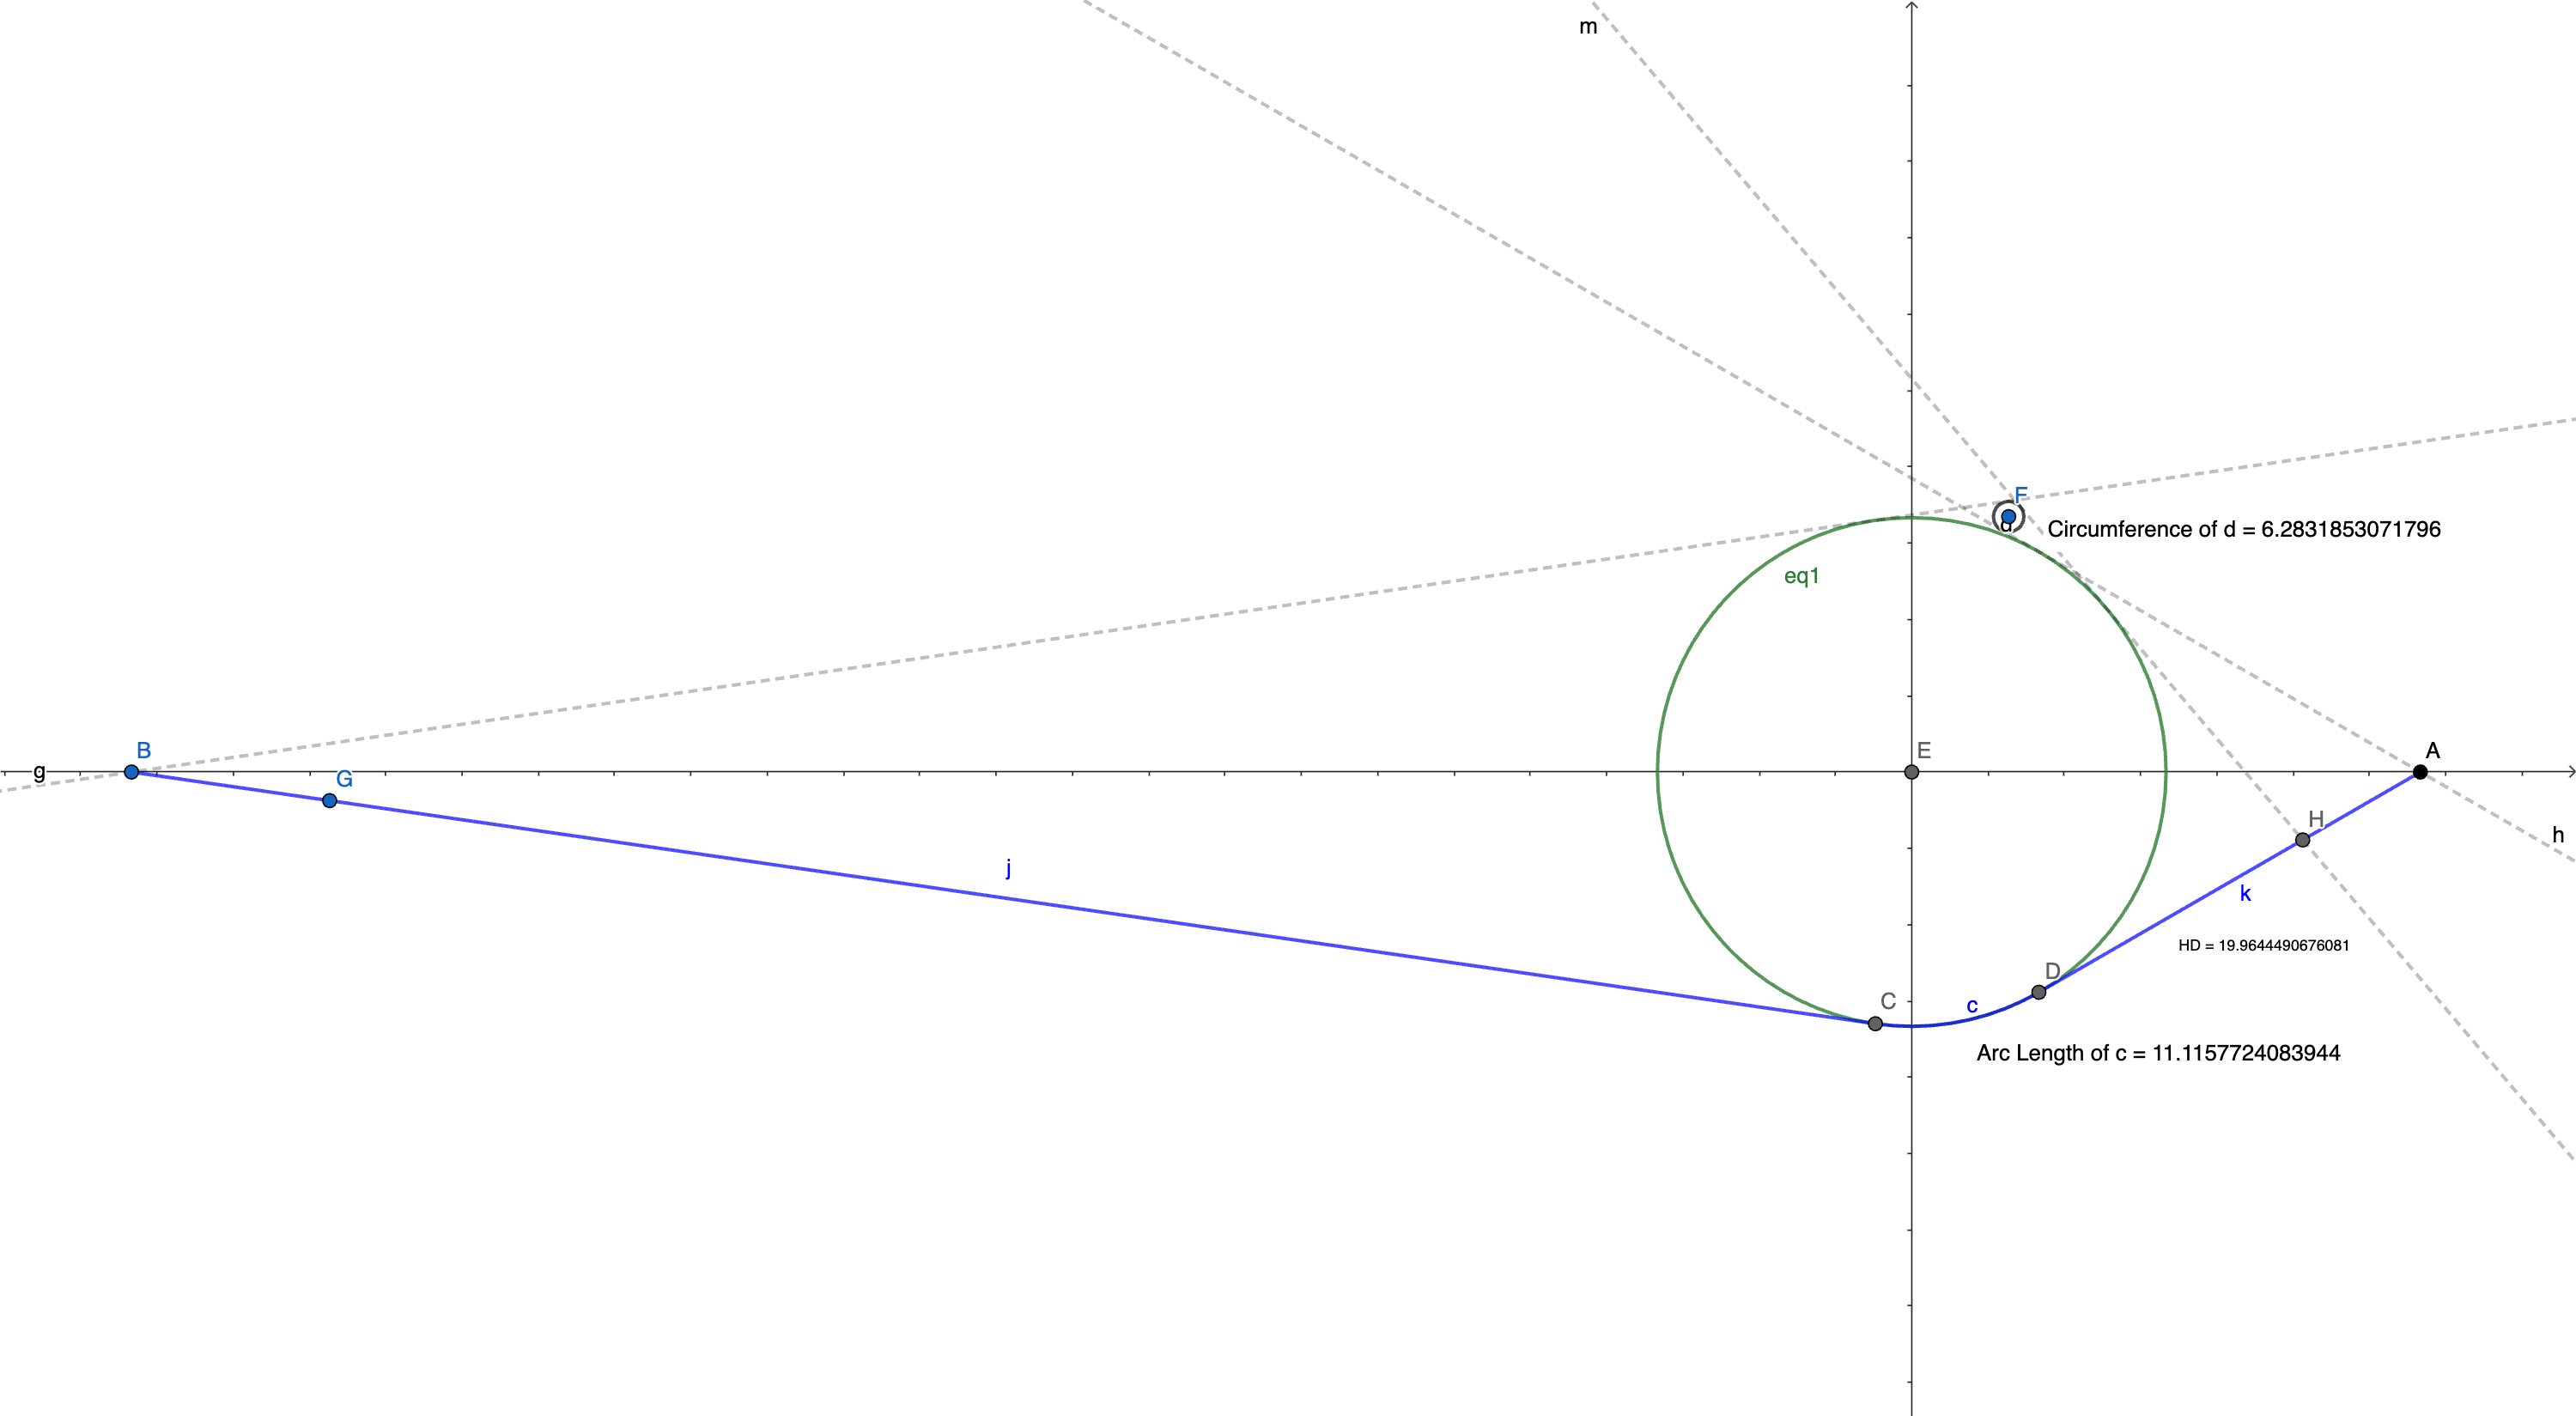
\includegraphics[width=\textwidth]{whole.png}
    \caption{轨迹}
    % \label{fig:PropProf}
\end{sidewaysfigure}
\begin{sidewaysfigure}[ht]
    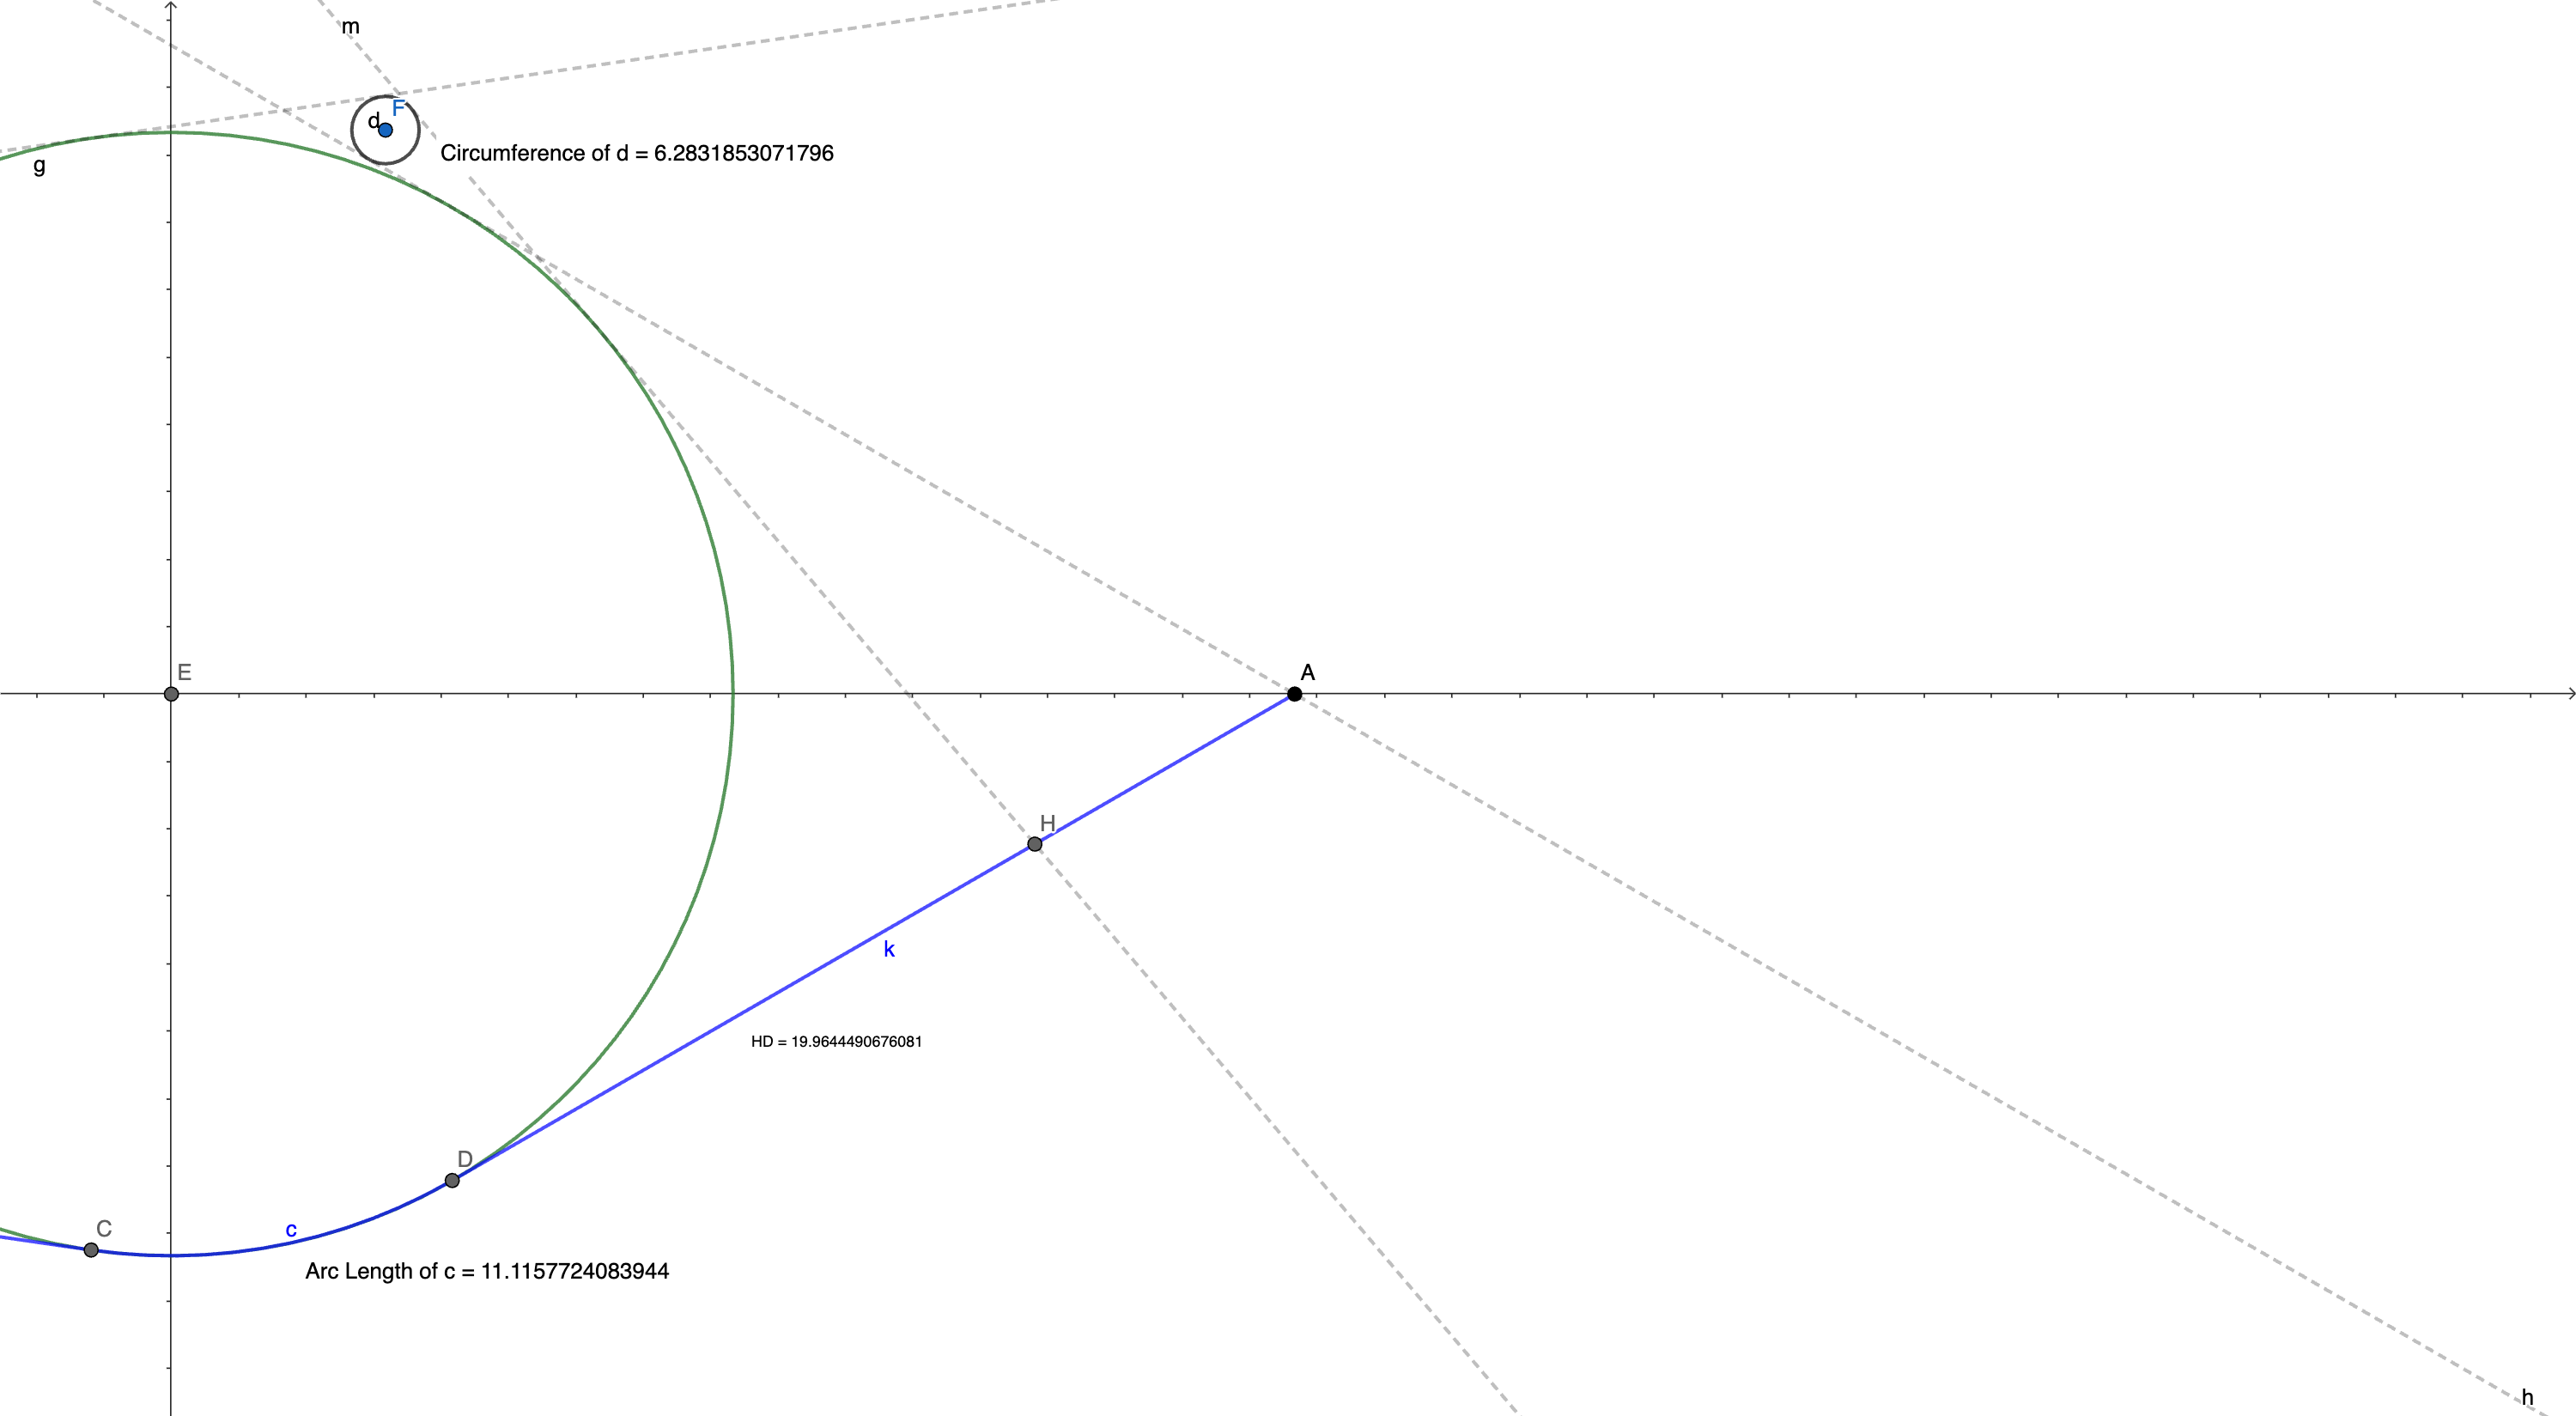
\includegraphics[width=\textwidth]{part.png}
    \caption{B避障估计}
    % \label{fig:PropProf}
\end{sidewaysfigure}




% \subsection{模型建立}



% \begin{enumerate}
% \item min\min\limits_{u_1, u_2} \min{t_1,t_2}
% \item \min\limits_{u_1, u_2} \max{t_1,t_2}\min\limits_{u_1, u_2} \max{t_1,t_2}
% \end{enumerate}

% \textbf{Control variables:}
% \begin{align*}
% u_1 &= \vec{a_1} \\
% u_2 &= \vec{a_2}
% \end{align*}

% \textbf{Subject to:}
% \begin{align*}
% r_1 &= z_1 = A \\
% r_2 &= z_2 = B \\
% |z_i| &\geq \frac{50}{3} \\
% z_1(0) &= \frac{100}{3} \\
% z_2(0) &= \frac{350}{3} \\
% \frac{\Im(z_1\bar{z_2})}{|z_1-z_2|} &\leq \frac{100}{3} \\
% |v_i| &= 1 \\
% \frac{1}{\kappa} &\geq 1 \\
% \kappa &\leq 1 \\
% |a_i| &\leq 1
% \end{align*}





% $$
% E = mc^2
% $$

% 引用公式\cref{eq:公式1}。

% \begin{equation}
% \label{eq:公式1}
% E = mc^2
% \end{equation}

% 引用\cref{fig:单图}。

% \begin{figure}[ht]
% \centering
% 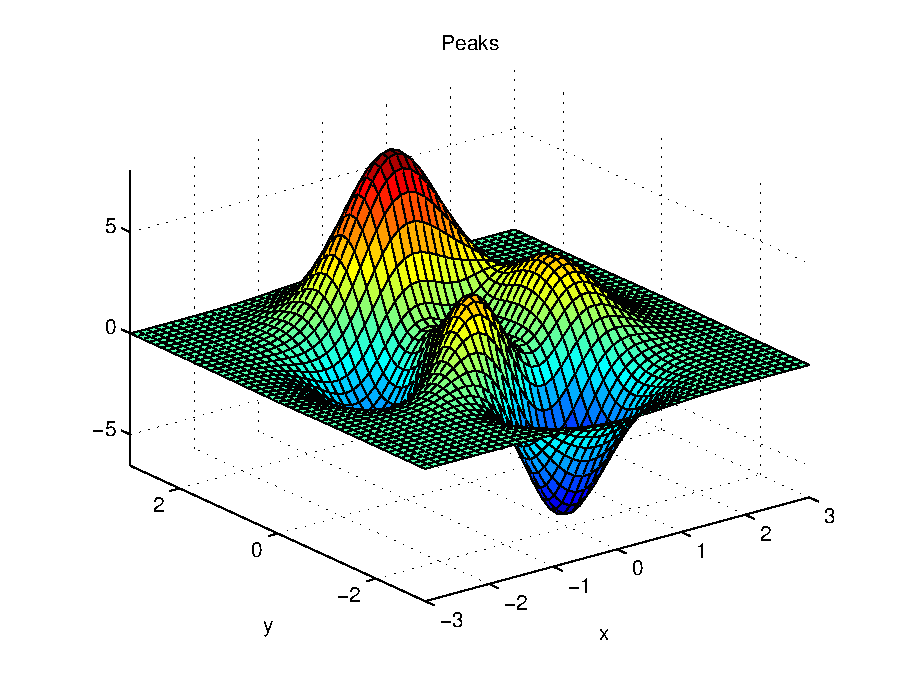
\includegraphics[width=0.75\textwidth]{example.eps}
% \caption{单图}
% \label{fig:单图}
% \end{figure}

% 这句话引用了文献\cite{司守奎2011数学建模算法与应用}。

% 这句话引用了文献\upcite{卓金武2011MATLAB}。

% \subsection{模型求解}

% \textbf{Step1:} 

% \textbf{Step2:} 

% \textbf{Step3:} 

% \subsection{求解结果}


%%%%%%%%%%%%%%%%%%%%%%%%%%%%%%%%%%%%%%%%%%%%%%%%%%%%%%%%%%%%% 

% \section{问题二的模型的建立和求解}
% \subsection{模型建立}

% 引用\cref{fig:双图},引用\cref{fig:双图a},引用\cref{fig:双图b}。

% \begin{figure}[ht]
% \centering
% \subcaptionbox{双图a子标题\label{fig:双图a}}
% {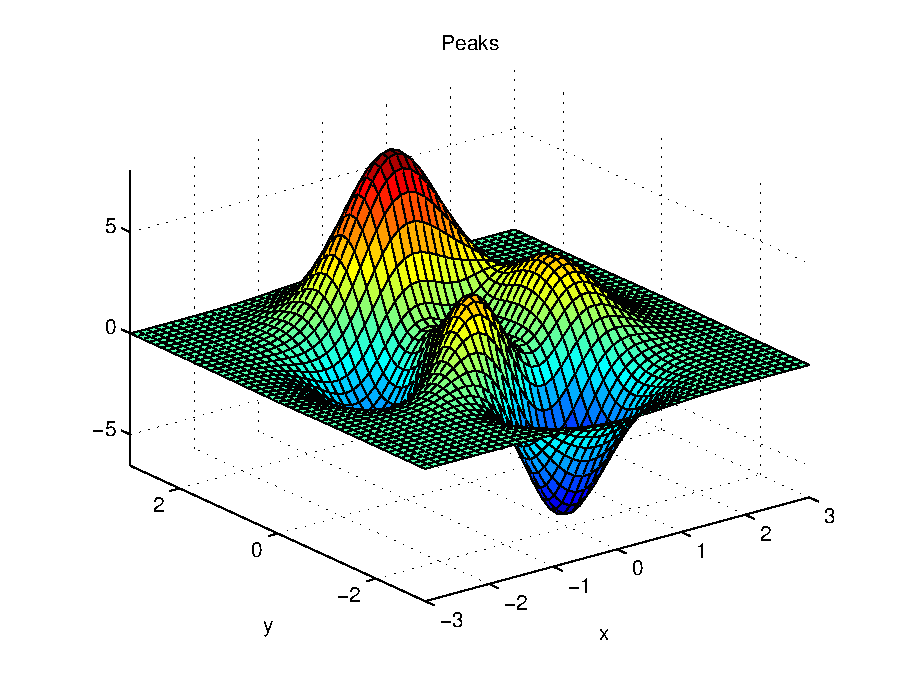
\includegraphics[width=.4\textwidth]{example.eps}}
% \subcaptionbox{双图b子标题\label{fig:双图b}}
% {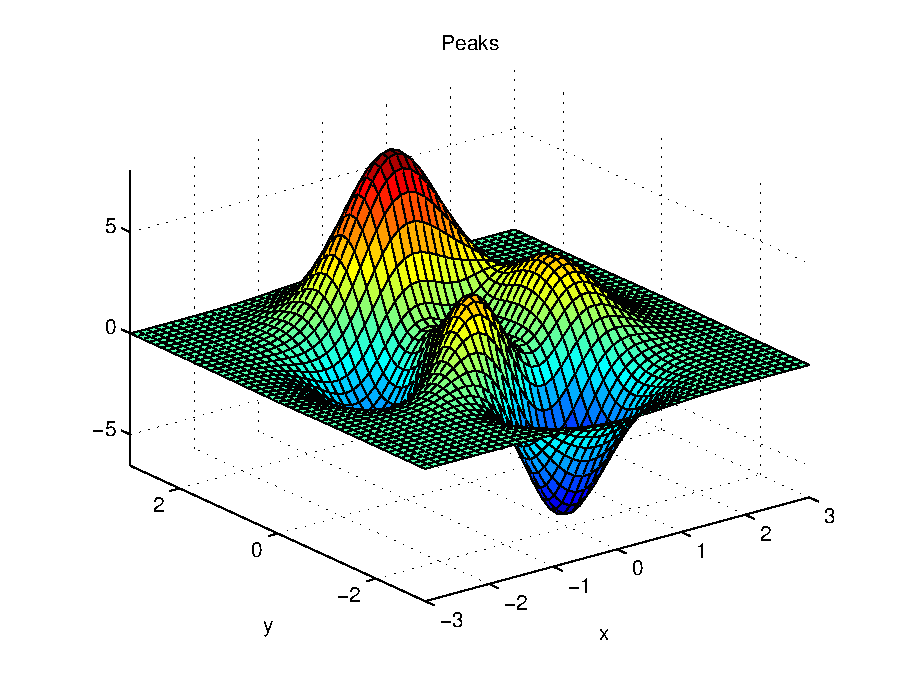
\includegraphics[width=.4\textwidth]{example.eps}}
% \caption{双图}\label{fig:双图}
% \end{figure} 

% \subsection{模型求解}

% \textbf{Step1:} 

% \textbf{Step2:} 

% \textbf{Step3:} 

% \subsection{求解结果}

% %%%%%%%%%%%%%%%%%%%%%%%%%%%%%%%%%%%%%%%%%%%%%%%%%%%%%%%%%%%%% 

% \section{问题三的模型的建立和求解}
% \subsection{模型建立}

% \subsection{模型求解}

% \textbf{Step1:} 

% \textbf{Step2:} 

% \textbf{Step3:} 

% \subsection{求解结果}

% %%%%%%%%%%%%%%%%%%%%%%%%%%%%%%%%%%%%%%%%%%%%%%%%%%%%%%%%%%%%% 

% \section{问题四的模型的建立和求解}
% \subsection{模型建立}

% \subsection{模型求解}

% \textbf{Step1:} 

% \textbf{Step2:} 

% \textbf{Step3:} 

% \subsection{求解结果}

% %%%%%%%%%%%%%%%%%%%%%%%%%%%%%%%%%%%%%%%%%%%%%%%%%%%%%%%%%%%%%

% \section{模型的分析与检验}

% \subsection{灵敏度分析}

% \subsection{误差分析}

% %%%%%%%%%%%%%%%%%%%%%%%%%%%%%%%%%%%%%%%%%%%%%%%%%%%%%%%%%%%%%

% \section{模型的评价}

% \subsection{模型的优点}
% \begin{itemize}[itemindent=2em]
% \item 优点1
% \item 优点2
% \item 优点3
% \end{itemize}

% \subsection{模型的缺点}
% \begin{itemize}[itemindent=2em]
% \item 缺点1
% \item 缺点2
% \end{itemize}

% %%%%%%%%%%%%%%%%%%%%%%%%%%%%%%%%%%%%%%%%%%%%%%%%%%%%%%%%%%%%%
% %% 参考文献
% \nocite{*}
% \bibliographystyle{gbt7714-numerical}  % 引用格式
% \bibliography{ref.bib}  % bib源

% \newpage
% %%%%%%%%%%%%%%%%%%%%%%%%%%%%%%%%%%%%%%%%%%%%%%%%%%%%%%%%%%%%%
% %% 附录
% \begin{appendices}
% \section{文件列表}
% \begin{table}[H]
% \centering
% \begin{tabularx}{\textwidth}{LL}
% \toprule
% 文件名   & 功能描述 \\
% \midrule
% q1.m & 问题一程序代码 \\
% q2.py & 问题二程序代码 \\
% q3.c & 问题三程序代码 \\
% q4.cpp & 问题四程序代码 \\
% \bottomrule
% \end{tabularx}
% \label{tab:文件列表}
% \end{table}

% \section{代码}
% \noindent q1.m
% \lstinputlisting[language=matlab]{code/q1.m}
% q2.py
% \lstinputlisting[language=python]{code/q2.py}
% q3.c
% \lstinputlisting[language=c]{code/q3.c}
% q4.cpp
% \lstinputlisting[language=c++]{code/q4.cpp}
% \end{appendices}
\end{document}


%%%%%双图模板%%%%%%
% \begin{figure}
% \centering
% \subcaptionbox{炉温曲线示意图\label{fig:双图a}}
% {\includegraphics[width=.4\textwidth]{炉温曲线示意图.png}}
% \subcaptionbox{问题1炉温曲线\label{fig:双图b}}
% {\includegraphics[width=.4\textwidth]{问题1炉温曲线.png}}
% \caption{双图}\label{fig:双图}
% \end{figure} 
%%%%%双图模板%%%%%%